\documentclass[tikz,border=7pt]{standalone}
\usepackage{amsmath,amssymb}
\usetikzlibrary{arrows.meta,patterns,decorations.markings,calc}
\tikzset{outline/.style={line width=.7pt,line cap=round,line join=round},
 map/.style={outline,-{Stealth[length=2.1mm,width=1.5mm]}},
 point/.style={circle,draw,fill=white,inner sep=1.4pt,line width=.6pt},
 along/.style={postaction={decorate},decoration={markings,mark=at position .52 with {\arrow{Stealth[length=1.8mm,width=1.2mm]}}}}}
\begin{document}
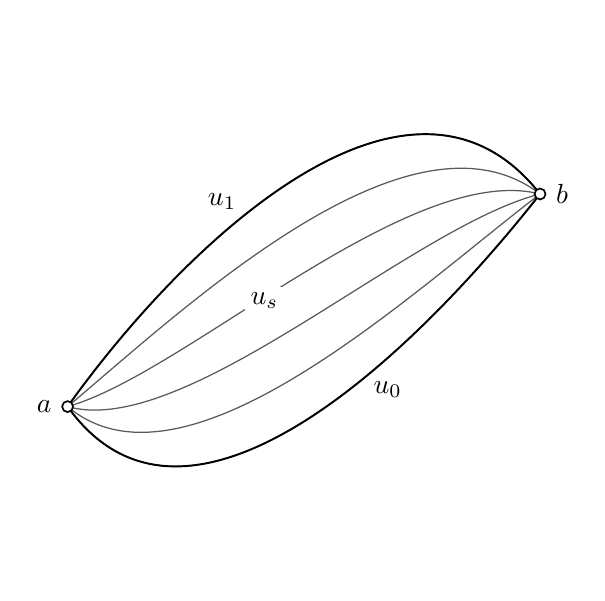
\begin{tikzpicture}[font=\normalsize]

\coordinate (a) at (0,0);\coordinate (b) at (6,2.7);
\foreach \s in {0,.2,.4,.6,.8,1}{
\pgfmathsetmacro{\h}{-2.1+4.2*\s}
\draw[line width=.45pt,black!65] (a) .. controls (1.5,\h) and (4.35,{2.7+\h}) .. (b);}
\draw[outline] (a) .. controls (1.5,-2.1) and (4.35,.6) .. (b) node[pos=.67,below=5pt] {$u_0$};
\draw[outline] (a) .. controls (1.5,2.1) and (4.35,4.8) .. (b) node[pos=.35,above=5pt] {$u_1$};


\node[fill=white,inner sep=2pt] at (2.5,1.35) {$u_s$};
\node[point,label=left:$a$] at (a) {};\node[point,label=right:$b$] at (b) {};

\end{tikzpicture}
\end{document}
